\documentclass[11pt, letterpaper]{article}
\usepackage{graphicx}
\usepackage[margin=1in]{geometry}
\usepackage{fancyhdr}
\usepackage[T1]{fontenc}
\usepackage{tabularx}
\usepackage[table, dvipsnames]{xcolor}
\usepackage{amssymb}
\usepackage{tikz}

\let\oldemptyset\emptyset
\let\emptyset\varnothing

\pagestyle{fancy}
\renewcommand{\headrulewidth}{0pt}

\fancyhf{}
\fancyfoot[R]{\thepage}

\begin{document}

\noindent Riley Rice\\CS321\\11-1-2024

\begin{center}\noindent {\Huge \textbf{Homework 3}}\end{center}

\section*{Problem 1: [10 points]}

\noindent For each of the language below, construct a regular expression that represents this language. All languages are over alphabet $\sum = {a,b}$.

\vspace{5mm}

\noindent In addition to the regular expression itself, provide a brief explanation (1-3 sentences) of the idea behind your construction. 

\vspace{5mm}

\noindent\textbf{Hint:} Sometimes you might need to deal with $\epsilon$ and single-character strings ($a$ and $b$) as special cases...

\vspace{5mm}

\noindent \textbf{(a)} The language is $\{w | w$ does NOT end with $aa\}$. For example, $\epsilon, a$, and $aaba$ are in the language, while $baa$ and $babaa$ are not.

\vspace{5mm}

\noindent\textbf{Solution:}
 
\vspace {5mm}

\noindent Answer

\vspace {5mm}

\noindent \textbf{Explanation:}

\vspace{5mm}

\noindent Answer

\vspace{5mm}

\noindent \textbf{(b)} The language is $\{w |$  the first and last characters of $w$ are different$\}$. For example, $abab$, and $bbbaa$ are in the language, while $\epsilon, a$ and $bbbbab$ are not.

\vspace{5mm}

\noindent\textbf{Solution:}
 
\vspace {5mm}

\noindent Answer

\vspace {5mm}

\noindent \textbf{Explanation:}

\vspace{5mm}

\noindent Answer

\newpage

\section*{Problem 2: [5 points]}

\noindent Let $L = \{a^mba^n | m \geq n\}$. For example, $b$, $aaba$, and $aaabaaa$ are in the language, while $\epsilon$, $aabba$, and $abaaa$ are not. Use the pumping lemma to prove that $L$ is not a regular language over alphabet $\sum = \{a, b\}$.

\vspace{5mm}

\noindent \textbf{Hint:} If you get stuck, reviewing the last example in Lec 13 might help.

\vspace{5mm}

\noindent\textbf{Solution:}

\vspace{5mm}

\noindent Answer

\newpage

\section*{Problem 3: [5 points]}

Give a regular expression equivalent to the following NFA (in fact it is a DFA).

\vspace{5mm}

\noindent I encourage you to write down the intermediate steps in addition to your final answer, so that you might get partial credits even if the final answer is wrong. (If your submission only includes the final answer, then it’s either 5 points or 0 points.)

\vspace{5mm}

\noindent \textbf{Hint:} As discussed in class, the very first step should be adding a "dummy" starting state and a separate "dummy" accepting state; this is not strictly necessary but it's error-prone if you don't do this.

\vspace{5mm}

\begin{center}
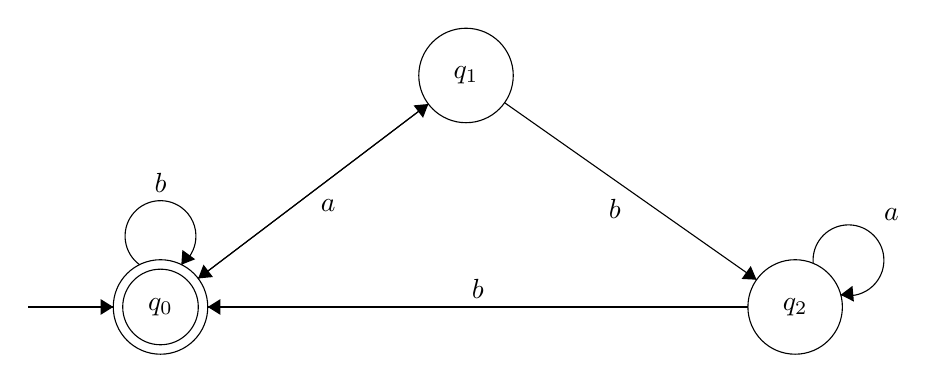
\begin{tikzpicture}[scale=0.2]
\tikzstyle{every node}+=[inner sep=0pt]
\draw [black] (8.6,-18) circle (3);
\draw (8.6,-18) node {$q_0$};
\draw [black] (8.6,-18) circle (2.4);
\draw [black] (28,-3.3) circle (3);
\draw (28,-3.3) node {$q_1$};
\draw [black] (48.9,-18) circle (3);
\draw (48.9,-18) node {$q_2$};
\draw [black] (0.2,-18) -- (5.6,-18);
\fill [black] (5.6,-18) -- (4.8,-17.5) -- (4.8,-18.5);
\draw [black] (7.277,-15.32) arc (234:-54:2.25);
\draw (8.6,-10.75) node [above] {$b$};
\fill [black] (9.92,-15.32) -- (10.8,-14.97) -- (9.99,-14.38);
\draw [black] (45.9,-18) -- (11.6,-18);
\fill [black] (11.6,-18) -- (12.4,-18.5) -- (12.4,-17.5);
\draw (28.75,-17.5) node [above] {$b$};
\draw [black] (50.046,-15.24) arc (185.18593:-102.81407:2.25);
\draw (54.52,-12.1) node [right] {$a$};
\fill [black] (51.79,-17.23) -- (52.63,-17.66) -- (52.54,-16.66);
\draw [black] (30.45,-5.03) -- (46.45,-16.27);
\fill [black] (46.45,-16.27) -- (46.08,-15.4) -- (45.5,-16.22);
\draw (37.45,-11.15) node [below] {$b$};
\draw [black] (10.99,-16.19) -- (25.61,-5.11);
\fill [black] (25.61,-5.11) -- (24.67,-5.2) -- (25.27,-5.99);
\draw (19.25,-11.15) node [below] {$a$};
\draw [black] (25.61,-5.11) -- (10.99,-16.19);
\fill [black] (10.99,-16.19) -- (11.93,-16.1) -- (11.33,-15.31);
\end{tikzpicture}
\end{center}

\vspace{5mm}

\noindent\textbf{Solution:}

\vspace{5mm}

\noindent Answer

\end{document}
